\documentclass[11pt,a4paper,twocolumn]{article}
\usepackage[cm]{fullpage}
\usepackage{newtxmath}
\usepackage{newtxtext}
\usepackage{graphicx}
\usepackage{hyperref}
\usepackage{placeins}

\begin{document}
\title{Networked Systems (H) Exercise 1}
\author{2785209M}
\maketitle

\subsection*{Question 1}
\begin{flushleft}
IP Address of Client: 130.209.247.112 \\
IP Address of Server: 93.93.131.127
\end{flushleft}

\section*{Question 2}
\begin{flushleft}
Client seq: 2687265183 \\
Server Seq: 2648910570
\end{flushleft}

\section*{Question 3}
\begin{flushleft}
Round Trip Time: 0.013717 seconds
\end{flushleft}

\section*{Question 4}
\begin{flushleft}
An acknowledgement in the TCP protocol is a signal sent from the receiver to the transmitter to indicate that a packet of data has been received.
When a connection is established an acknowledgement handshake between the client and the server must be performed. The client transmits a random initial sequence number (SYN),
the server receives this and sends back an acknowledgement alongside its own random sequence number (SYN-ACK), and finally the client sends back its own acknowledgement (ACK), completing the handshake.
Once the hanshake is completed the client and server can each send and recieve data. In standard TCP, if data is sent but no acknowledgement is received, it creates a timeout.
This indicates packet loss and causes the transmitter to go backwards, retransmitting packets until it recieves acknowledgement of the missing packet. This can take time. TCP selective acknowledgement improves TCP congestion control by removing
the necessity to retransmit large sequences of data. If one piece of data is missing, the receiver will send an ACK telling the transmitter what it has, and what it doesn't have. This allows the transmitter to only retransmit what is needed.
This improves the efficiency of congestion control in TCP, requiring less bandwidth, using less energy, and taking less time.
\end{flushleft}

\section*{Question 5}
\begin{flushleft}
The TCP receive window is a period of time in which the receiver tells the transmitter how many bytes of data it can receive per ACK cycle, in order to prevent it being overwhelmed with packets. 
This ensures that the transmitter does not transmit data faster than the receiver can process it.
The size of the receive window can be calculated by multiplying the raw window value by the window scaling factor. 
From the receiver's side, the raw window value in this example is 65535 (which is the max) and the window scaling factor is 6, which gives a window size of 393210 Bytes.
\end{flushleft}

\section*{Question 6}
\begin{flushleft}
The receive window is a receiver-side limit on how much data it can receive at a time to prevent the receiver from being overwhelmed.
The congestion window is a server-side limit on how much data is can send over the netork to avoid overwhelming the network.
Both of these factors can limit TCP throughput. The throughput will be limited by whichever window is smaller.
\end{flushleft}

\section*{Question 7}
\begin{flushleft}
An acknowledgement is sent back as soon as data is received even if the data is still being processed by the server to prevent the client from thinking the packet was lost.
\end{flushleft}

\section*{Question 8}
\begin{flushleft}
During a Server Hello the server sends three unique data packets simultaneously. These include the Cipher Suite, a Public Key, and Server Random Data. 
These files are large and so must be split between multiple packets.
\end{flushleft}

\section*{Question 9}
\begin{flushleft}
Packets 9-13 contain the end of the TLS handshake, and the beginning of data transfer.
\end{flushleft}

\section*{Question 10}
\begin{flushleft}
    See Figure 1.
\end{flushleft}

\section*{Question 11}
\begin{flushleft}
This plot shows clear evidence of the TCP slow start. In the TCP the size of the packets sent is increased every round trip. 
At the beginning the packet size doubles every RTT, increasing exponentially.
At about 0.17 seconds congestion control kicks in and slows down the growth to a linear progression to prevent congestion.
\\ Behaviours shown: TCP slow start and TCP congestion avoidance.
\end{flushleft}

\section*{Question 12}
\begin{flushleft}
At approximately 0.2 seconds there is a noticeable drop in the sequence number. This indicates a packet loss and retransmission event. 
It also demonstrates TCP fast recovery as transmission does not restart from zero, but jumps back a bit and continues transmitting normally.
\\ Behaviours shown: Packet Loss and TCP fast recovery.
\end{flushleft}


\FloatBarrier
\onecolumn

\section*{Appendix}
\begin{figure}[h!]
    \centering
    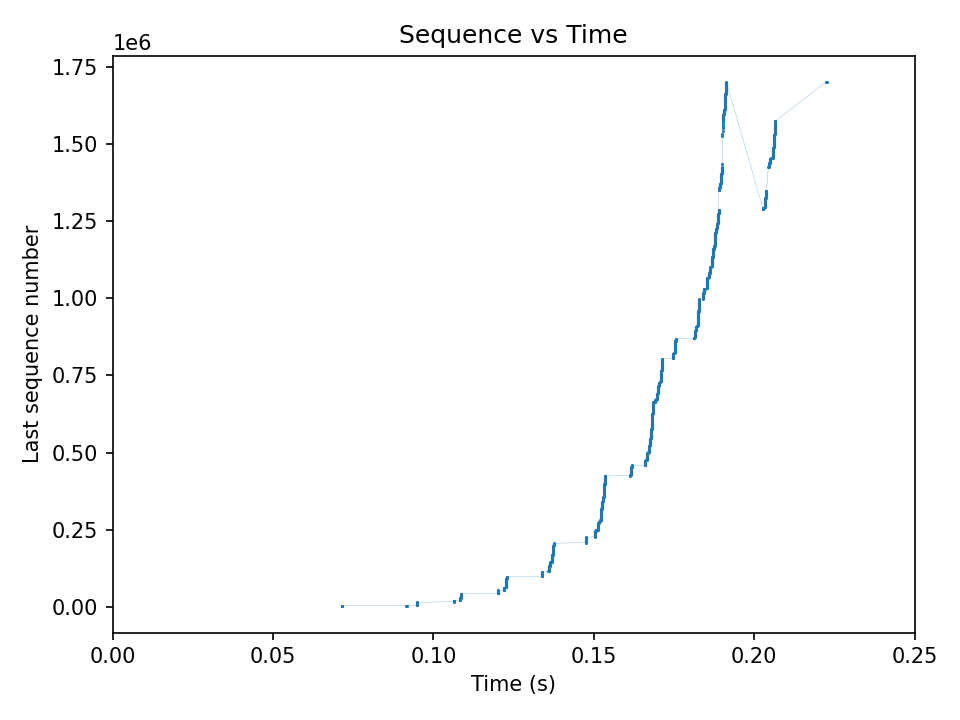
\includegraphics[scale=1]{plot.png}
    \caption{Plot of TCP sequence number over time}
\end{figure}

\section*{References}
\begin{flushleft}
https://www.tcpdump.org/index.html\\
https://tls13.xargs.org/\\
https://dev-aditya.medium.com/tls-over-tcp-protocols-how-secure-internet-connections-really-work-4c4addc30801
\end{flushleft}

\end{document}